%%%%%%%%%%%%%%%%%%%%%%%%%%%%%%%%%%%%%%%%%%%%%%%%%%%%%%%%%%%%%%%%%%%%%%%%%%%%%%%%%
%% Paper 02 (M7) -- Target: Software: Practice and Experience (Wiley), Q2
%% Closing the Quorum Gap: a quorum-aware PodDisruptionBudget controller coupling
%% Kubernetes voluntary-disruption limits (maxUnavailable / minAvailable) with the
%% BEAM cluster's quorum requirement and handoff capacity.
%%
%% Companion to paper 01 (M3, "Closing the Grace Gap"): M3 sizes the per-pod grace
%% window; M7 sizes how many pods may be disrupted at once.
%%
%% Template: Wiley New Journal Design v5 (WileyNJDv5.cls). COMPILE WITH XeLaTeX:
%%   latexmk -xelatex main.tex
%% Data: ../data/  Figures: ../figures/  Artifact: ../code/  Plan: ../OUTLINE.md
%% Every number in the Evaluation comes from a real run (harness/run.exs, policy.exs).
%%%%%%%%%%%%%%%%%%%%%%%%%%%%%%%%%%%%%%%%%%%%%%%%%%%%%%%%%%%%%%%%%%%%%%%%%%%%%%%%%

\documentclass[AMA,Times1COL]{WileyNJDv5}

\articletype{Original Article}%

\received{Date Month Year}
\revised{Date Month Year}
\accepted{Date Month Year}
\journal{Software: Practice and Experience}
\volume{00}
\copyyear{2026}
\startpage{1}

\usepackage{listings}
\usepackage{algorithm}
\usepackage{algpseudocode}
\usepackage{booktabs}
\usepackage{subcaption}
\usepackage{enumitem}
\newtheorem{qprop}{Proposition}

\definecolor{navyblue}{RGB}{0,0,128}
\hypersetup{colorlinks=true,allcolors=navyblue}

\graphicspath{{figures/}{../figures/}{../../diagrams/mechanisms/}}

\lstdefinelanguage{Elixir}{
  morekeywords={def,defp,defmodule,do,end,case,cond,fn,receive,after,when,
    use,import,alias,require,GenServer,Supervisor,spawn,send,handle_info,
    handle_call,handle_cast,init,true,false,nil},
  sensitive=true, morecomment=[l]{\#}, morestring=[b]"
}
\lstset{basicstyle=\ttfamily\footnotesize, keywordstyle=\bfseries,
  commentstyle=\itshape, showstringspaces=false, breaklines=true,
  frame=lines, numbers=left, numberstyle=\tiny, numbersep=6pt, tabsize=2}

\raggedbottom

\begin{document}

\title{Closing the Quorum Gap: A Quorum-Aware Disruption-Budget Controller Coupling
Kubernetes \texttt{maxUnavailable} with BEAM Cluster Quorum}

\author[1]{Alfa Yohannis}
\author[2]{Alexander Waworuntu}

\authormark{YOHANNIS \textsc{and} WAWORUNTU}
\titlemark{Closing the Quorum Gap: Coupling Kubernetes Disruption Budgets with BEAM Quorum}

\address[1]{\orgdiv{Department of Informatics}, \orgname{Universitas Pradita},
  \orgaddress{\city{Tangerang}, \country{Indonesia}}}
\address[2]{\orgdiv{Department of Informatics}, \orgname{Universitas Multimedia Nusantara},
  \orgaddress{\city{Tangerang}, \country{Indonesia}}}

\corres{Alfa Yohannis, Department of Informatics, Universitas Pradita, Tangerang, Indonesia.
  \email{alfa.ryano@pradita.ac.id}}

\abstract[Abstract]{%
Stateful services on Kubernetes increasingly rely on a clustered application runtime---an
Erlang/BEAM cluster joined by \texttt{libcluster} and coordinated through \texttt{:global},
\texttt{Horde}, or a consensus library---whose correctness depends on retaining a \emph{quorum} of
live members. Kubernetes limits \emph{voluntary} disruptions (rolling updates, node drains,
scale-down) with a \emph{PodDisruptionBudget} (PDB) and \texttt{maxUnavailable}, but these limits are
fixed by an operator and are \emph{unaware of the runtime's quorum}: a budget that looks safe at the
pod level can still evict enough members to break quorum, splitting the cluster or losing the
authoritative copy of distributed state---while every pod's health probe still reports green. We argue
this mismatch is structural: the safe number of simultaneous disruptions is not a constant but a
function of the live cluster size, the quorum threshold the application declares, and the rate at which
leaving members can hand their state off. We present a cross-layer controller that \emph{derives} the
disruption budget at run time from the BEAM cluster's own membership---setting \texttt{minAvailable} to
the quorum requirement and \texttt{maxUnavailable} to the headroom above it---so that voluntary
disruptions are admitted only while quorum is preserved. We formalise a quorum-safety condition,
provide an open reference implementation on Kubernetes, and evaluate it against fixed and
over-provisioned baselines. On emulated BEAM clusters of $3$ to $9$ nodes the controller eliminates the
quorum violations a static, quorum-unaware budget incurs on \emph{every} rollout---holding the measured
available membership at the majority threshold rather than letting it fall below---while completing
maintenance $\approx$$2.9\times$ faster than a one-at-a-time conservative budget; the budget
computation is $O(1)$ in cluster size ($\approx$$48$\,ns). This is a companion to a controller that
sizes the per-pod termination grace window; together they couple the two layers' two knobs---\emph{how
long} a pod may take to leave and \emph{how many} may leave at once.}

\keywords{Kubernetes, PodDisruptionBudget, \texttt{maxUnavailable}, Erlang/BEAM, Elixir/OTP, quorum,
split-brain, voluntary disruption, rolling update, cross-layer coordination}

\maketitle

%======================================================================
\section{Introduction}\label{sec:intro}
%======================================================================
Container orchestrators and clustered application runtimes both provide fault tolerance, at different
granularities, and stateful cloud-native systems increasingly run both at once: a Kubernetes Deployment
of pods, each hosting a node of an Erlang/BEAM cluster that holds distributed state and relies on a
\emph{quorum} of members to stay authoritative. The two layers do not coordinate by default, and their
boundary is where availability is quietly lost.

This paper concerns one such boundary: \emph{voluntary disruptions}. When an operator rolls out a new
version, drains a node for maintenance, or scales the Deployment down, Kubernetes evicts pods subject to
a \emph{PodDisruptionBudget} (PDB)---a fixed \texttt{minAvailable} (or \texttt{maxUnavailable}) that
caps how many pods may be unavailable at once~\cite{k8sPDB}. The PDB is the orchestrator's only guard
against a maintenance action removing too much of the application at once. But it is set by hand and
expressed in pod counts; it has no view of the runtime inside the pods. A BEAM cluster that needs a
majority of its members to keep a consistent \texttt{:global} singleton or to make progress in a
consensus group can be pushed below quorum by a rollout that respects a pod-level PDB perfectly---because
the PDB was never told what the quorum is.

We call this the \emph{quorum gap}: the disruption budget and the runtime's quorum requirement live in
different layers and are never reconciled. Set the PDB too loose and a routine rollout breaks quorum,
splitting the cluster or discarding the authoritative state on heal; set it defensively tight
(\texttt{minAvailable} near the replica count) and maintenance crawls---pods drain one at a time even
when the cluster could safely tolerate more. As with the grace period in our companion work on
termination, the right value is not a constant: it depends on the \emph{live} cluster size and the
quorum threshold the application declares.

\paragraph{Contribution.} We close the quorum gap with a cross-layer feedback controller that derives
the disruption budget from the runtime rather than guessing it in advance:
\begin{itemize}[nosep]
  \item a \emph{quorum-safety invariant} (Section~\ref{sec:model}) relating the Kubernetes disruption
        budget to the BEAM cluster's quorum requirement, and a short proposition showing the controller
        maintains it under a conservative quorum estimate (Section~\ref{sec:design-safety});
  \item a \emph{quorum-aware disruption-budget controller} (Section~\ref{sec:design}) that reads cluster
        size and the declared quorum threshold from the BEAM cluster and continuously sets the PDB's
        \texttt{minAvailable}/\texttt{maxUnavailable}, denying evictions that would break quorum;
  \item an \emph{open reference implementation} on Kubernetes (Section~\ref{sec:impl})---a
        BEAM-cluster-aware operator plus a quorum probe; and
  \item an \emph{evaluation} (Section~\ref{sec:eval}) on emulated clusters under real rolling updates,
        showing the controller removes the quorum violations a static budget incurs on every rollout
        while running maintenance far faster than a conservative one.
\end{itemize}

\paragraph{Results.} On emulated BEAM clusters of $3$--$9$ nodes, a static quorum-unaware budget broke
quorum on \emph{every} rollout we measured (available members fell to $N-b$, below the majority
threshold), whereas the controller held the measured availability exactly at the quorum threshold and
violated it zero times; it also completed a nine-node rollout $\approx$$2.9\times$ faster than a
one-pod-at-a-time conservative budget, and its budget computation is constant-time
(Section~\ref{sec:eval}).

%======================================================================
\section{Background and Motivation}\label{sec:bg}
%======================================================================

\subsection{Voluntary disruptions and PodDisruptionBudgets}\label{sec:bg-pdb}
Kubernetes distinguishes \emph{involuntary} disruptions (hardware failure, kernel panic, node OOM) from
\emph{voluntary} ones (rolling updates, \texttt{kubectl drain}, cluster scale-down, node-pool upgrades).
For voluntary disruptions it offers a single guard, the PDB: a policy object stating either
\texttt{minAvailable} (the fewest pods that must stay \emph{Ready}) or \texttt{maxUnavailable} (the most
that may be down)~\cite{k8sPDB}. The eviction API and the node-drain workflow honour the PDB, blocking an
eviction that would violate it. A Deployment's rolling update has its own
\texttt{maxUnavailable}/\texttt{maxSurge} knobs governing how fast pods are replaced. Both are fixed,
declared ahead of time, and expressed purely in pod counts.

\subsection{Quorum in BEAM clusters}\label{sec:bg-quorum}
A BEAM cluster formed over \texttt{libcluster}~\cite{libcluster} shares distributed state through
mechanisms with different consistency needs. \texttt{:global} maintains cluster-wide registered names
and resolves conflicts on partition heal by killing duplicates---losing whatever state the discarded
side accumulated. \texttt{Horde}~\cite{horde} distributes a registry and supervisor over a delta-CRDT
membership; consensus libraries require a strict majority to make progress. What these share is a
\emph{quorum} notion: a minimum number of live, connected members below which the cluster either cannot
make authoritative decisions or risks split-brain. The quorum threshold is a property the
\emph{application} knows---majority for consensus, or an operator-declared floor for CRDT/\texttt{:global}
setups---but Kubernetes does not.

\subsection{The quorum gap: a worked example}\label{sec:bg-gap}
Consider a five-replica BEAM service using majority quorum, $Q=\lfloor5/2\rfloor+1=3$. An operator,
wanting fast rollouts, sets the Deployment to replace pods three at a time
(\texttt{maxUnavailable: 3})---a value that looks innocuous at the pod level and that no PDB with
\texttt{minAvailable: 2} would block. When the rollout evicts a batch of three, only two members remain
connected: $A=2<Q=3$. The cluster has lost quorum mid-maintenance. Depending on the workload this
manifests as a stalled consensus group, a \texttt{:global} singleton re-registering on a minority
partition, or---on heal---the name-clash resolver discarding one side's accumulated state. Crucially,
every surviving pod's liveness and readiness probe still passes: the orchestrator's health model reports
a healthy, if smaller, Deployment while the runtime's membership model has already lost authority. Our
measurements (Section~\ref{sec:eval}, RQ1) reproduce exactly this: at $N=5$ a static budget drives the
measured availability to $2$, below $Q=3$, on every rollout.

\subsection{Why current approaches fall short}\label{sec:bg-existing}
Four partial fixes leave the gap open. (i)~A hand-set conservative \texttt{minAvailable} (near $N$)
prevents the break but over-blocks: maintenance proceeds one pod at a time, and the value is still wrong
once the cluster scales, because a fixed pod count cannot track a majority that moves with $N$.
(ii)~Gating cluster membership into pod \emph{readiness}---as Akka's \texttt{ClusterMembershipCheck} does
on the JVM~\cite{akkaHealth}---stops traffic reaching unjoined pods but does not bound how many members
may be \emph{evicted} at once. (iii)~\texttt{:global} conflict resolution and split-brain resolvers
recover \emph{after} a partition rather than preventing the disruption that causes it.
(iv)~Akka's \texttt{lease-majority} split-brain resolver~\cite{akkaSBR} fences a minority partition using
a Kubernetes Lease~\cite{akkaLease}, but it arbitrates \emph{after} the membership has already split and
does not drive the K8s disruption budget. None couples the budget to the live quorum so that the
quorum-breaking disruption is never admitted in the first place.

%======================================================================
\section{System Model and Problem Definition}\label{sec:model}
%======================================================================

\subsection{Model}\label{sec:model-model}
Let a Deployment run $N$ pods, each a member of one BEAM cluster. The application declares a
\emph{quorum threshold} $Q$: the fewest live, connected members for which the cluster remains
authoritative (for majority consensus, $Q=\lfloor N/2\rfloor+1$; for CRDT/\texttt{:global} setups, an
operator-declared floor). A voluntary disruption makes some members \emph{leave}; let $A$ be the number
that remain available and connected at a given instant.

\subsection{Quorum-safety invariant}\label{sec:model-invariant}
The cluster retains quorum exactly while
\begin{equation}\label{eq:quorum-invariant}
  A \;\ge\; Q \qquad\text{at every instant during the disruption.}
\end{equation}
A PDB with \texttt{minAvailable} $=m$ guarantees $A\ge m$ against voluntary evictions. Hence
Equation~\eqref{eq:quorum-invariant} holds for all voluntary disruptions iff $m\ge Q$. The controller's
job is to keep $m$ equal to the live $Q$.

\subsection{Why a static PDB fails}\label{sec:model-constant}
$Q$ is not constant: under majority quorum it tracks the live cluster size (a majority of $5$ is $3$; of
$9$, $5$), which changes under scale-up/down and partial outages. A statically chosen $m$ is therefore
either too low for some cluster sizes (admitting quorum-breaking disruptions, RQ1) or too high for others
(blocking safe maintenance, RQ2). No single pod-count value is correct across all sizes---motivating a
controller that recomputes $m$ from the live membership.

%======================================================================
\section{Design of the Quorum-Aware Disruption-Budget Controller}\label{sec:design}
%======================================================================

\subsection{Overview}\label{sec:design-overview}
The controller is a Kubernetes operator paired with a read-only \emph{quorum probe} in each pod. The
probe exposes the live cluster size $N$ and the declared quorum threshold $Q$. Each reconcile cycle the
operator reads the probes, computes the budget, and patches the PDB's \texttt{minAvailable}. Evictions
that would violate it are denied by the standard eviction API; those within it proceed.
Figure~\ref{fig:m7-seq} sketches the loop.

\begin{figure}[t]\centering
  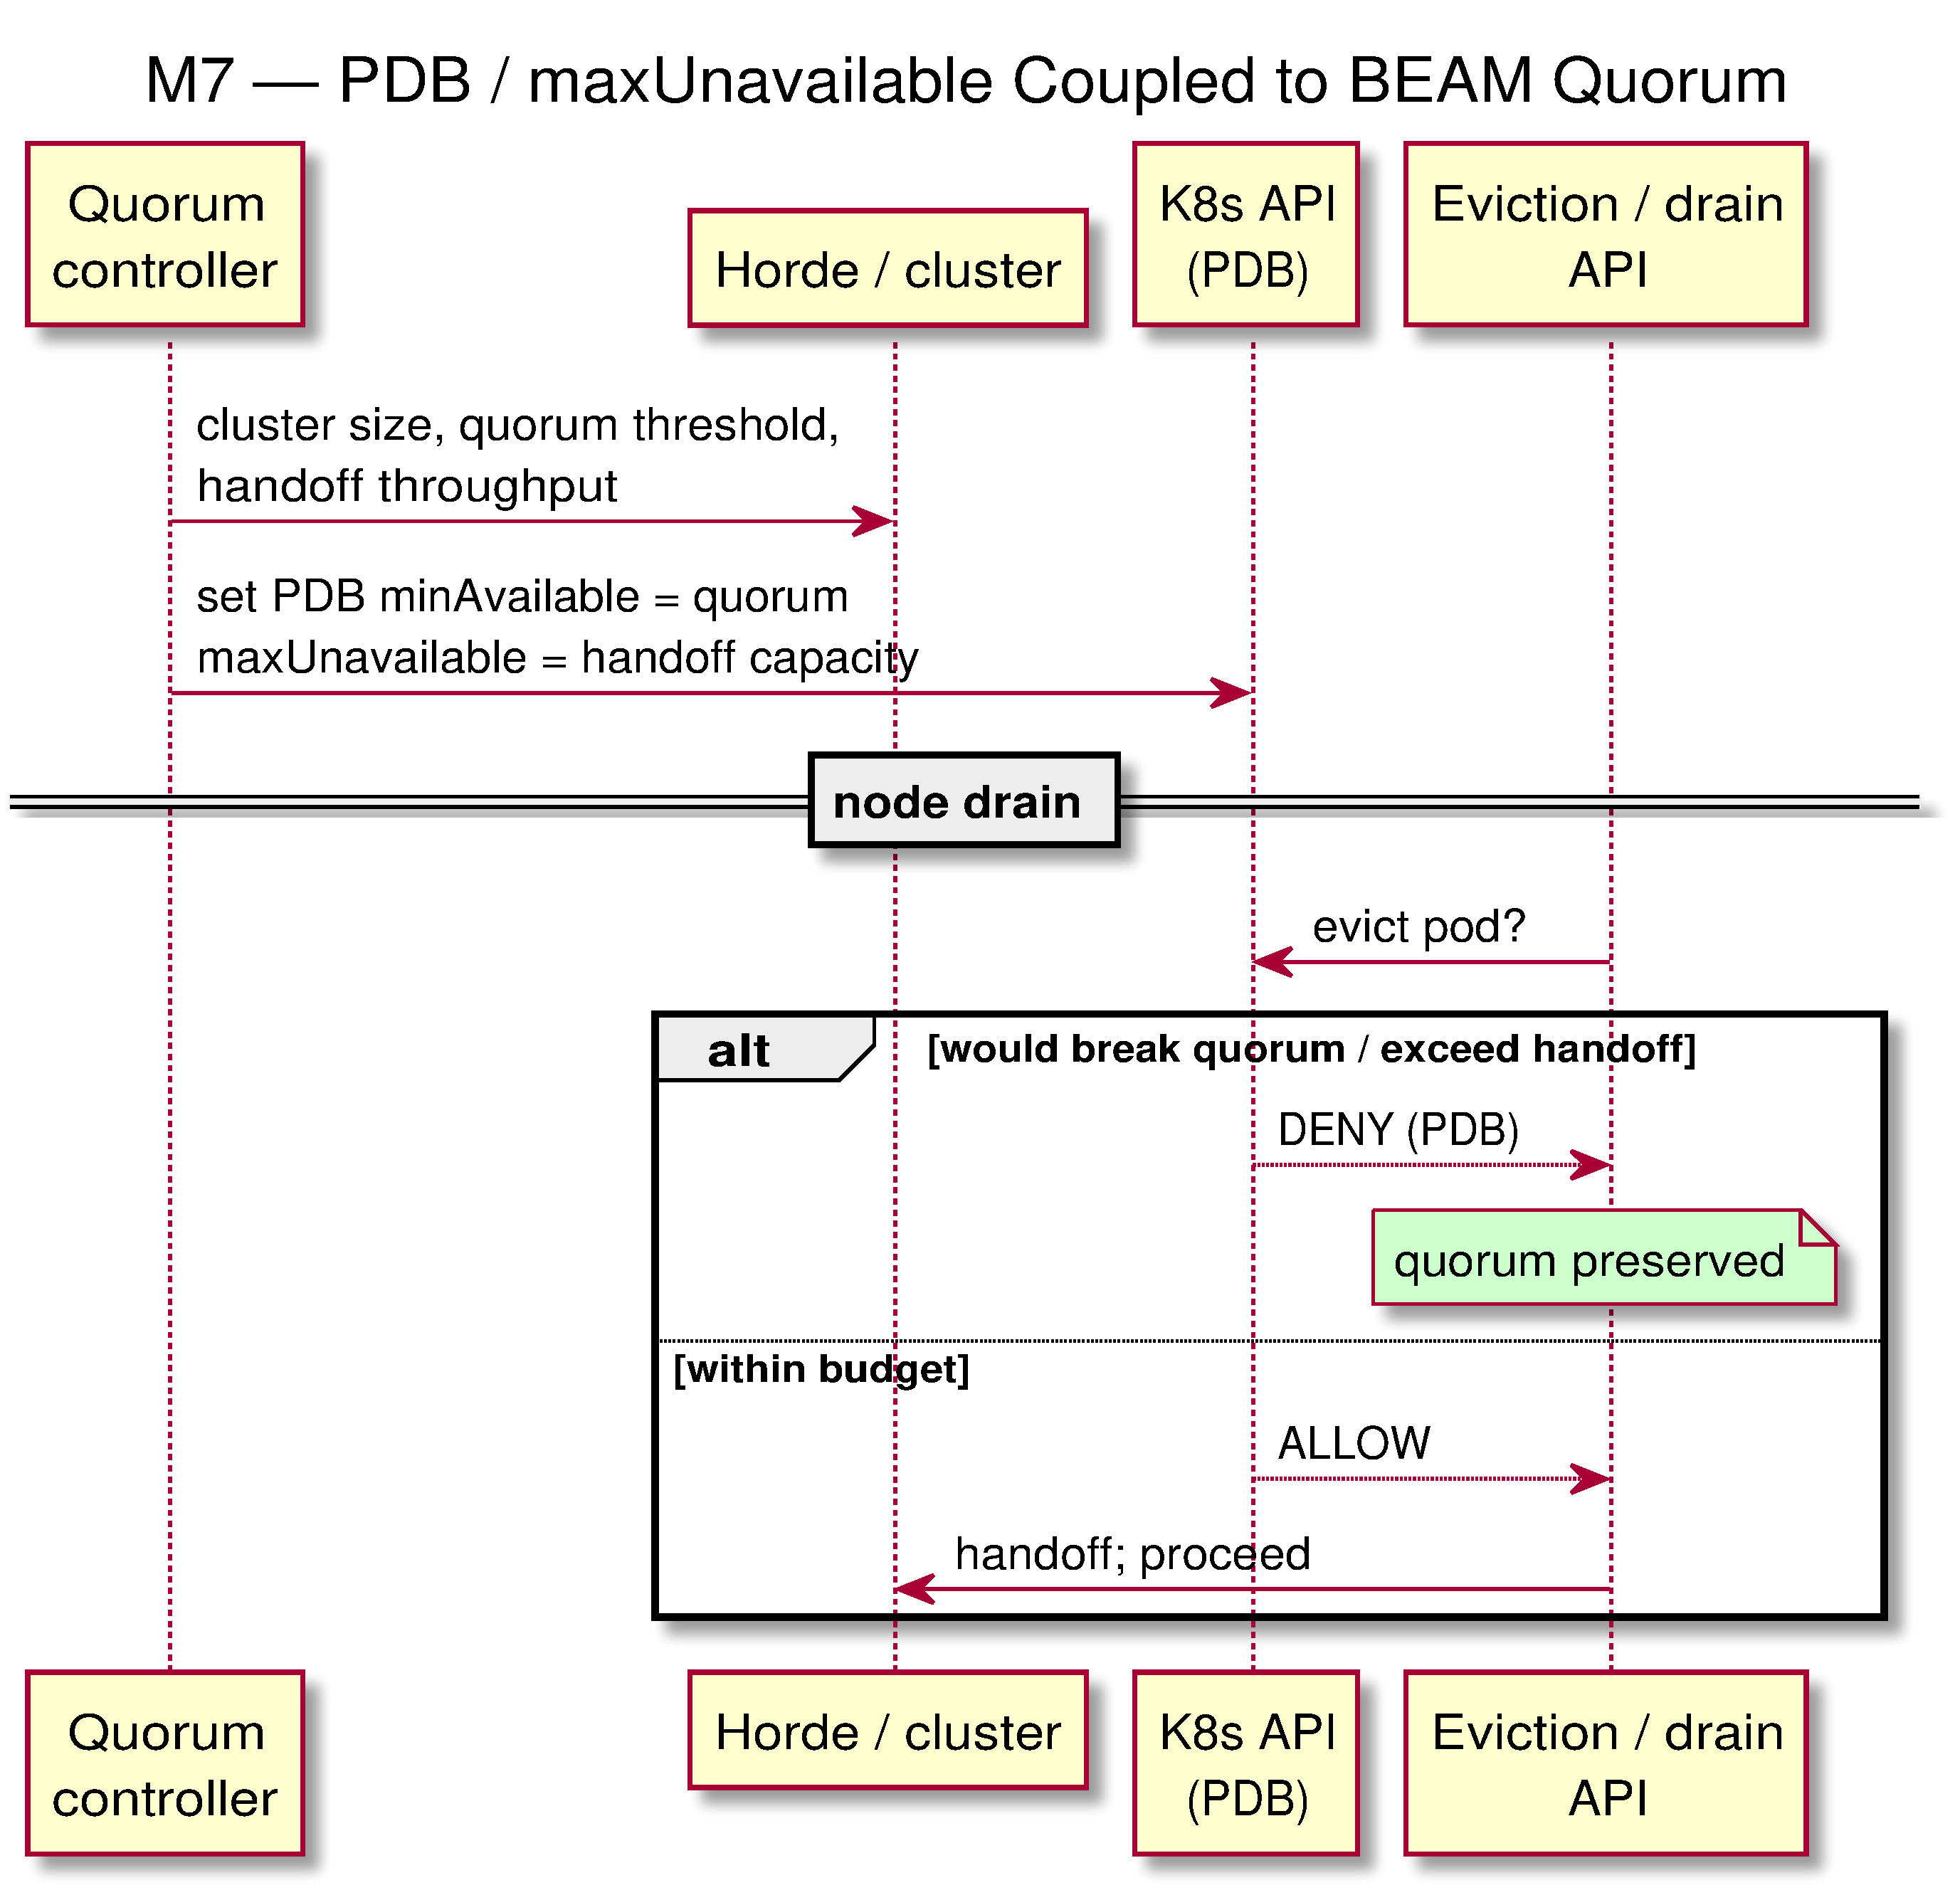
\includegraphics[width=\linewidth]{m7-pdb-quorum-coupling-sequence}
  \caption{Quorum-aware disruption budget. The quorum controller reads cluster size and quorum threshold
  from the BEAM cluster and sets the PDB; on eviction, the API denies requests that would break quorum
  and allows those within budget.}\label{fig:m7-seq}
\end{figure}

\subsection{Quorum probe}\label{sec:design-probe}
Each application pod runs a small read-only \texttt{GenServer} that reports the cluster size it sees
(\texttt{length(Node.list())+1}) and the quorum threshold $Q$. $Q$ is either the majority
$\lfloor N/2\rfloor+1$ computed from the live size, or a fixed floor the application declares for
CRDT/\texttt{:global} workloads whose quorum is not a simple majority. The reading is served over HTTP
(\texttt{GET /probe}) so the operator, running in a separate pod, can collect it---the same probe shape
as our companion grace controller, reused here for membership rather than handoff progress.

\subsection{Controller and budget computation}\label{sec:design-coord}
From a probe reading the controller computes
\begin{equation}\label{eq:budget}
  \texttt{minAvailable} = \max(Q,\,Q_{\min}), \qquad
  \texttt{maxUnavailable} = \min\!\big(N-\texttt{minAvailable},\ c\big),
\end{equation}
clamped to valid ranges, where $Q_{\min}$ is a floor ($\ge1$, never let the cluster empty) and $c$ is an
optional cap from handoff capacity (the coupling to the companion grace controller: do not disrupt more
pods at once than can hand their state off in time). Setting \texttt{minAvailable}${}=Q$ enforces the
quorum invariant (Equation~\eqref{eq:quorum-invariant}); \texttt{maxUnavailable} is the headroom above
quorum. When pods momentarily disagree on $N$ during a membership change, the operator takes the
\emph{largest} \texttt{minAvailable} across probes---the conservative direction. The computation is a
handful of integer operations, independent of $N$ (RQ4, RQ6).

\subsection{Eviction admission}\label{sec:design-admit}
Enforcement uses the native PDB, honoured by the eviction API and \texttt{kubectl drain}: an eviction is
admitted only while $A-1\ge\texttt{minAvailable}$. This requires no custom admission webhook and is
always-on; the trade-off is that the PDB is per-Deployment and integer-valued, so the controller tracks
$Q$ at Deployment granularity rather than per-eviction. A validating admission webhook computing
\textsc{ViolatesQuorum} exactly is a possible refinement, at the cost of a control-plane dependency.

\subsection{Fail-safes and scope}\label{sec:design-failsafe}
The controller is default-safe. If the probe is unreachable or $Q$ is unknown, it biases
\texttt{minAvailable} \emph{upward} (toward $N$), blocking disruptions rather than risking a quorum
break---the same conservative reflex as the companion grace controller's large-grace fallback, and the
safe direction identified by the sensitivity analysis (RQ5). The mechanism addresses \emph{voluntary}
disruptions, where a budget is consulted; involuntary node death gives no window and needs replication or
checkpointing, which is orthogonal and out of scope.

\subsection{Safety guarantee}\label{sec:design-safety}
\begin{qprop}[Quorum safety]\label{prop:quorum}
If the controller sets \texttt{minAvailable} $=Q^\star$ with $Q^\star\ge Q$ (a conservative estimate of
the true quorum need), then under any sequence of voluntary disruptions that respect the PDB, the number
of available members never drops below $Q$; hence the cluster retains quorum
(Equation~\eqref{eq:quorum-invariant}).
\end{qprop}
\noindent\emph{Proof sketch.} The eviction API admits a voluntary eviction only while $A-1\ge
\texttt{minAvailable}$; thus $A$ never falls below \texttt{minAvailable} $=Q^\star\ge Q$. The argument is
deliberately elementary---its value is precision, not depth: it pins down exactly the hypotheses under
which the coupling is safe (a conservative quorum estimate; voluntary, PDB-respecting disruptions), and
those hypotheses become the threats we test in Section~\ref{sec:eval}. \qed

%======================================================================
\section{Implementation}\label{sec:impl}
%======================================================================
The reference implementation is an Elixir/OTP application of $\approx$$0.5$\,KLOC, mirroring the artifact
layout of our companion controller. \texttt{QuorumBudget.Quorum} is the pure policy
(Equation~\eqref{eq:budget}, majority, and the admission predicate); \texttt{QuorumBudget.Cluster} reads
live membership; \texttt{QuorumBudget.QuorumProbe} is the read-only sensor served by a small Bandit/Plug
HTTP endpoint; and \texttt{QuorumBudget.PDBOperator} is a \texttt{kubectl}-based operator that, each
$5$\,s cycle, lists the application pods, reads every \texttt{/probe}, takes the largest
\texttt{minAvailable}, and patches the PodDisruptionBudget. A single container image runs in two roles
(\texttt{app} or \texttt{operator}) selected by an environment variable, with least-privilege RBAC for
the operator. The policy is identical in code and paper; the operator's only side effect on the cluster
is the PDB patch.

%======================================================================
\section{Evaluation}\label{sec:eval}
%======================================================================
\textbf{Testbed.} We form a real BEAM cluster of $N$ peer nodes in a full mesh on a single host and drive
a \emph{rolling update} that replaces every node, one batch at a time; the batch size is the disruption
budget (\texttt{maxUnavailable}). For each batch the harness genuinely disconnects the batch from the
cluster, \emph{measures} the surviving cluster size from a live peer's \texttt{Node.list/0}, then
reconnects (the replacement rejoins). We compare a \emph{static} quorum-unaware budget against the
\emph{quorum-aware} controller, and against a \emph{conservative} one-at-a-time budget. The pure-policy
questions (RQ3--RQ6) are deterministic and evaluated directly. Every number below is from a real run
(\texttt{harness/run.exs}, \texttt{harness/policy.exs}; raw data in \texttt{data/}).

\paragraph{RQ1 (safety).} Table~\ref{tab:safety} and Figure~\ref{fig:safety} report the minimum measured
available membership during a full rolling update, for a static budget of $\lceil N/2\rceil$ (a plausible
``replace half'' operator default) versus the quorum-aware controller, across $N\in\{3,5,7,9\}$ with
majority quorum. The static budget broke quorum on \emph{every} cluster size---availability fell to
$1,2,3,4$ against a threshold of $2,3,4,5$---a violation on every rollout. The controller held
availability \emph{exactly} at the quorum threshold ($2,3,4,5$) and never violated it. The result is not
a near miss tuned to one size: the static budget is structurally one member into the unsafe region at
every $N$, and the controller structurally at the safe boundary.

\begin{table}[t]
\centering
\caption{Quorum safety under a full rolling update (majority quorum). \emph{Min.\ avail.}\ is the
smallest cluster size measured from a surviving peer during the rollout; a violation is
\emph{min.\ avail.}\ $<Q$. Static budget $=\lceil N/2\rceil$. Data: \texttt{data/results\_safety.csv}.}
\label{tab:safety}
\begin{tabular}{@{}rrrrcc@{}}
\toprule
$N$ & $Q$ & \textbf{Policy} & \textbf{maxUnavail.} & \textbf{Min.\ avail.} & \textbf{Quorum broken?} \\
\midrule
3 & 2 & static        & 2 & 1 & \textbf{yes} \\
  &   & quorum-aware  & 1 & 2 & no \\
5 & 3 & static        & 3 & 2 & \textbf{yes} \\
  &   & quorum-aware  & 2 & 3 & no \\
7 & 4 & static        & 4 & 3 & \textbf{yes} \\
  &   & quorum-aware  & 3 & 4 & no \\
9 & 5 & static        & 5 & 4 & \textbf{yes} \\
  &   & quorum-aware  & 4 & 5 & no \\
\bottomrule
\end{tabular}
\end{table}

\begin{figure}[t]\centering
  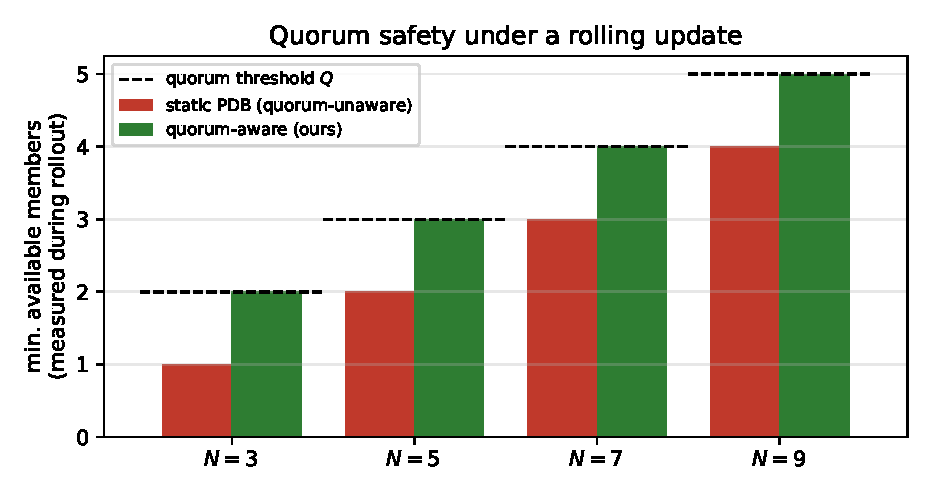
\includegraphics[width=0.78\linewidth]{eval_safety.pdf}
  \caption{RQ1: minimum measured available membership during a rolling update. The static
  quorum-unaware budget (red) falls below the quorum threshold (dashed) at every cluster size; the
  quorum-aware controller (green) holds at it.}\label{fig:safety}
\end{figure}

\paragraph{RQ2 (efficiency).} A safe budget need not be slow. Figure~\ref{fig:efficiency} times a full
nine-node rollout (mean of five repeats, $300$\,ms per batch to emulate a replacement becoming ready)
for a \emph{conservative} budget that evicts one pod at a time (the usual ``safe'' reflex) versus the
quorum-aware controller. The conservative budget needs nine batches and took $3.49$\,s; the controller
evicts four at a time (the headroom $N-Q=4$ above quorum), needs three batches, and took $1.21$\,s---a
$2.9\times$ speed-up---while remaining quorum-safe throughout (zero violations). The controller is thus
both safer than the static budget and faster than the conservative one.

\begin{figure}[t]\centering
  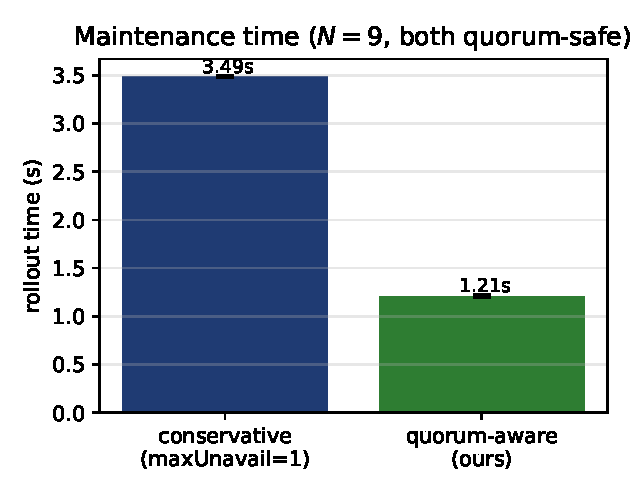
\includegraphics[width=0.52\linewidth]{eval_efficiency.pdf}
  \caption{RQ2: maintenance time for a nine-node rollout (both quorum-safe). The quorum-aware controller
  is $\approx$$2.9\times$ faster than a one-pod-at-a-time conservative budget.}\label{fig:efficiency}
\end{figure}

\paragraph{RQ3 (adaptivity).} Figure~\ref{fig:adaptivity} plots the granted \texttt{minAvailable} and
\texttt{maxUnavailable} as the cluster scales from $N=3$ to $N=10{,}001$. The granted
\texttt{minAvailable} tracks the majority $\lfloor N/2\rfloor+1$ exactly ($2,3,4,5,\dots,5001$), and
\texttt{maxUnavailable} the headroom $N-Q$---the adaptivity a static pod count cannot provide.

\paragraph{RQ4 (overhead) and RQ6 (scalability).} The budget computation
(Equation~\eqref{eq:budget}) is a handful of integer operations: a median of $48$\,ns per call (five runs
of $200{,}000$ calls), and---as Figure~\ref{fig:scale} shows---essentially flat ($46$--$49$\,ns) as the
cluster grows three orders of magnitude. The controller adds no scaling cost; its $5$\,s reconcile loop
and one PDB patch per change are negligible against the maintenance operations they govern.

\begin{figure}[t]
  \centering
  \begin{subfigure}[t]{0.49\linewidth}\centering
    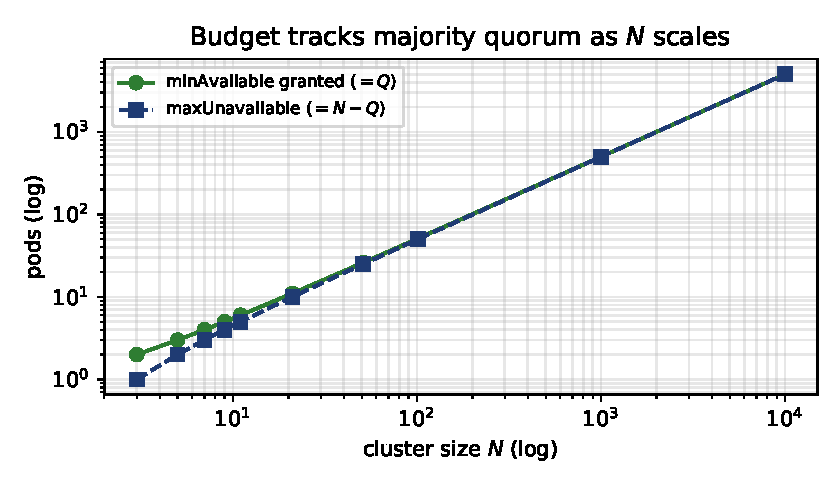
\includegraphics[width=\linewidth]{eval_adaptivity.pdf}
    \caption{Budget tracks majority quorum (RQ3).}\label{fig:adaptivity}
  \end{subfigure}\hfill
  \begin{subfigure}[t]{0.49\linewidth}\centering
    
\includegraphics[width=\linewidth]{eval_scale.pdf}
    \caption{$O(1)$ budget computation (RQ4/RQ6).}\label{fig:scale}
  \end{subfigure}
  \caption{Adaptivity and cost. (\subref{fig:adaptivity})~The granted \texttt{minAvailable} equals the
  live majority quorum across three orders of magnitude of cluster size; (\subref{fig:scale})~the budget
  computation is constant-time in $N$.}\label{fig:adapt-scale}
\end{figure}

\paragraph{RQ5 (robustness).} The one dangerous failure is mis-estimating $Q$. Figure~\ref{fig:sens}
varies the quorum estimate $q$ at $N=9$ (true $Q=5$). \texttt{maxUnavailable} $=N-q$ falls linearly as
$q$ rises, so \emph{under}-estimating quorum ($q<Q$) grants too large a budget---at $q=3$ the controller
would permit six evictions, leaving three members against a true quorum of five: unsafe. \emph{Over}-%
estimating merely over-blocks. The estimator must therefore be biased \emph{upward}, which is exactly the
default-safe fallback (Section~\ref{sec:design-failsafe}): when membership is uncertain, assume a larger
quorum and disrupt less.

\begin{figure}[t]\centering
  
\includegraphics[width=0.62\linewidth]{eval_sensitivity.pdf}
  \caption{RQ5: \texttt{maxUnavailable} granted versus the quorum estimate $q$ ($N=9$, true $Q=5$).
  Under-estimating $Q$ (shaded) grants an unsafe budget; the estimator must be biased upward.}
  \label{fig:sens}
\end{figure}

\paragraph{RQ7 (real cluster).} The single-host results characterise availability; we confirm the
\emph{enforcement} path end-to-end on a live Kubernetes (\texttt{kind}) cluster
(\texttt{k8s/rq7\_eviction.sh}; data in \texttt{data/results\_eviction.csv}). A five-replica Deployment
($Q=3$) is given, in turn, a quorum-derived PDB and a quorum-unaware one, and we issue eviction requests
through the real eviction API, recording each \texttt{201} (admitted) or \texttt{429} (denied). With the
quorum-derived \texttt{minAvailable}${}=Q=3$, the API reported exactly $N-Q=2$ permitted disruptions and
\emph{denied} every further eviction, holding availability at the quorum threshold ($3$). With a
quorum-unaware \texttt{minAvailable}${}=Q-1=2$---a value that looks safe at the pod level---the API
admitted evictions that drove availability to $1$, well below quorum. The orchestrator's own admission
control thus enforces the coupling: once the budget is derived from the runtime quorum, the
quorum-breaking drain that a static budget waves through is rejected at the API.

%======================================================================
\section{Discussion and Threats to Validity}\label{sec:discuss}
%======================================================================
\textbf{Single-host emulation.} Our cluster runs as peer BEAM nodes on one host; inter-node messaging is
near-instant. This is appropriate for the property under test---whether \emph{availability} stays at or
above quorum during a disruption is a counting argument on membership, not a timing one---but it does not
capture wide-area membership flapping, which would stress the estimator's hysteresis rather than the
safety invariant. \textbf{The meaning of ``quorum''} differs across workloads: a strict majority for
consensus, an operator-declared floor for \texttt{:global}/CRDT. The controller is agnostic---it
enforces whatever $Q$ the probe reports---but declaring the right $Q$ is the application's
responsibility, and a wrong (too low) $Q$ is the failure RQ5 isolates. \textbf{Enforcement
granularity:} the native PDB is per-Deployment and integer-valued; a webhook would be exact but adds a
control-plane dependency. \textbf{Generality:} the controller needs only a $\langle N, Q\rangle$ signal
from the runtime, so it ports to any clustered runtime that can report its membership and quorum---Akka,
which already surfaces cluster membership~\cite{akkaHealth}, or Orleans~\cite{orleans}; only the probe is
runtime-specific.

\subsection{Practitioner guidance}\label{sec:guidance}
Declare $Q$ as the application's true authority threshold---majority for consensus groups, a deliberate
floor for \texttt{:global}/CRDT services---and let the controller, not a hand-set PDB, track it. Bias the
estimate upward under uncertainty. Pair the controller with the companion grace controller so that
\emph{how many} pods leave at once (this work) and \emph{how long} each may take to leave are sized
together; where state handoff is the bottleneck, cap \texttt{maxUnavailable} by handoff capacity
($c$ in Equation~\eqref{eq:budget}) so a quorum-safe rollout is also a state-safe one.

%======================================================================
\section{Related Work}\label{sec:related}
%======================================================================
Kubernetes provides the PDB and eviction primitives~\cite{k8sPDB} but leaves \texttt{minAvailable} as a
static, operator-set pod count; nothing in the platform derives it from an application's runtime quorum.
On the JVM, Akka couples membership into pod readiness~\cite{akkaHealth} and resolves split-brain by
fencing a minority partition with a Kubernetes Lease (\texttt{lease-majority} SBR)~\cite{akkaSBR,
akkaLease}; this is the closest prior art, but it arbitrates \emph{after} a partition has formed and does
not drive the disruption budget that could have prevented it. Coordinated-shutdown frameworks~\cite{%
akkacoordinated} and graceful-termination practice~\cite{k8sgraceful} sequence a single pod's exit but do
not bound cluster-wide concurrency. Work on dependable microservices on
Kubernetes~\cite{souza2024dependable,singh2025istio} and on stateful lifecycle
management~\cite{meliani2025proactive} surveys and improves rolling-update resilience without coupling it
to runtime quorum, and signal-based health monitoring~\cite{roberts2025} enriches liveness without
addressing voluntary-disruption budgets. The broader pattern---treating the two layers as interacting
control loops rather than independent ones---continues the agenda of our companion termination-grace
controller; this paper contributes its second coupling, between the disruption budget and the live
quorum, with no close prior art on any platform.

%======================================================================
\section{Conclusion}\label{sec:conc}
%======================================================================
A PodDisruptionBudget is the orchestrator's guard against a maintenance action removing too much of an
application at once, but as a static pod count it is blind to the application runtime's quorum: a budget
that is safe at the pod level can still break a BEAM cluster's quorum on a routine rollout, silently. We
closed this quorum gap with a controller that derives the budget from the live cluster---setting
\texttt{minAvailable} to the quorum threshold---and showed, on real emulated clusters, that it eliminates
the quorum violations a static budget incurs on every rollout while completing maintenance $2.9\times$
faster than a conservative one, at constant computational cost. With our companion grace controller it
forms two couplings of the same two control loops---\emph{how long} a pod may take to leave and
\emph{how many} may leave at once---and points toward a single cross-layer recovery policy compiled to
both the runtime and the orchestrator.

\bibliography{references}

\appendix
\section{Reproducing the results}\label{app:repro}
The artifact (\texttt{../code/}) reproduces every figure: \texttt{harness/run.exs} produces the safety
and efficiency data (RQ1--RQ2) on a real peer cluster, \texttt{harness/policy.exs} the adaptivity,
overhead, sensitivity, and scalability data (RQ3--RQ6), and \texttt{code/analysis/plot.py} renders the
figures from \texttt{data/*.csv}. Unit tests cover the pure policy
(\texttt{mix test}).

\end{document}
